\section{Enhancing network with physics information}
\par{}
The already developed neural network code was validated against two dataset,
and now the code has to be enhanced to include physics information in the form
of mathematical constraints.\\

\par{}
For each problem to be solved with this network code, the code has to be
modified to include the mathematical constraints in the last layer or so. The
mathematical constraints can be of two types, either algebraic or differential
equations. Algebraic equations involving output and input variables can be
directly coded, but, coding the differential equations will require the
derivatives to be computed using automatic differentiation in the network which
was accomplished as explained below.\\

\subsection{Computing derivatives output w.r.t input}
\par{}
The differential equations (ODEs and PDEs) will involve the
derivatives of dependent variables w.r.t. independent variables. In the
network terms, the dependent variables are the output variables and the
independent ones are the input variables. Thus, as similar to the loss derivative
equations, an equation for computing derivative of a layer output w.r.t. its
input was derived. \\

\par{}
Keeping backpropagation equations as base idea, the matrix equation for
\(\partial \sigma/\partial x\) of a layer was propertly derived and is given
below as.

\begin{align}
    \left[\frac{\partial \sigma}{\partial \bm{x}}\right] = \left[\bm{W}\right]^T \cdot diag\left(\frac{\partial \sigma}{\partial \bm{z}}\right) \label{differential_matrix_eqn}
\end{align}

\par{}
Here, \(\partial \sigma/\partial x\) is a vector of the layer and
\(diag\left(\partial \sigma/\partial x\right)\) is a diagonal matrix with those
vector elements on the diagonal.\(\left[\frac{\partial \sigma}{\partial
\bm{x}}\right] \) is a mtrix of same size as of \(\left[\bm{W}\right]^T\). \\

\par{}
It has to be noted that the \cref{differential_matrix_eqn} gives derivative
of output with respect to input of a single layer only. The chain rule in
differential calculus has to be used to get the derivative of overall output
of the network to its actual input.\\

\subsection{Validating the gradient equation}
\par{}
The matrix equation \cref{differential_matrix_eqn} was validated for it working
by testing it on the network that was trained based on pure data. A network
was built and trained using a synthetic data of fluid velocity decay at a point
in flow due to fluid viscosity. The synthetic data was generated using below equation
with \(k = 5.0\) and \(V_0 = 1\).

\begin{align*}
    V(t) = V_0 e^{-k t}
\end{align*}

And its corresponding ODE for derivative computation is given below.

\begin{align*}
    \frac{d V}{d t} = -k V
\end{align*}

\par{}
The network was trained for \(X = t = [0,0.5]\) and its corresponding velocity
values. The estimated vs exact velocity decay profile is given in
\cref{validation_decay_profile}.  And then, the trained layer weights were used
to compute the derivative \(d V/d t\) which were compared to the exact values
and given in \cref{validation_derivative_profile}.  It can be seen that the
derivative profiles match quite well except at the beginning which is due to
limitation in approximating the velocity profile, and that was later rectified
in validating the PINN network. Thus, the derivative computation is validated,
and next step will be to validate the self built physics-informed neural
network.

\begin{figure}
    \begin{subfigure}{0.5\linewidth}
       \center
        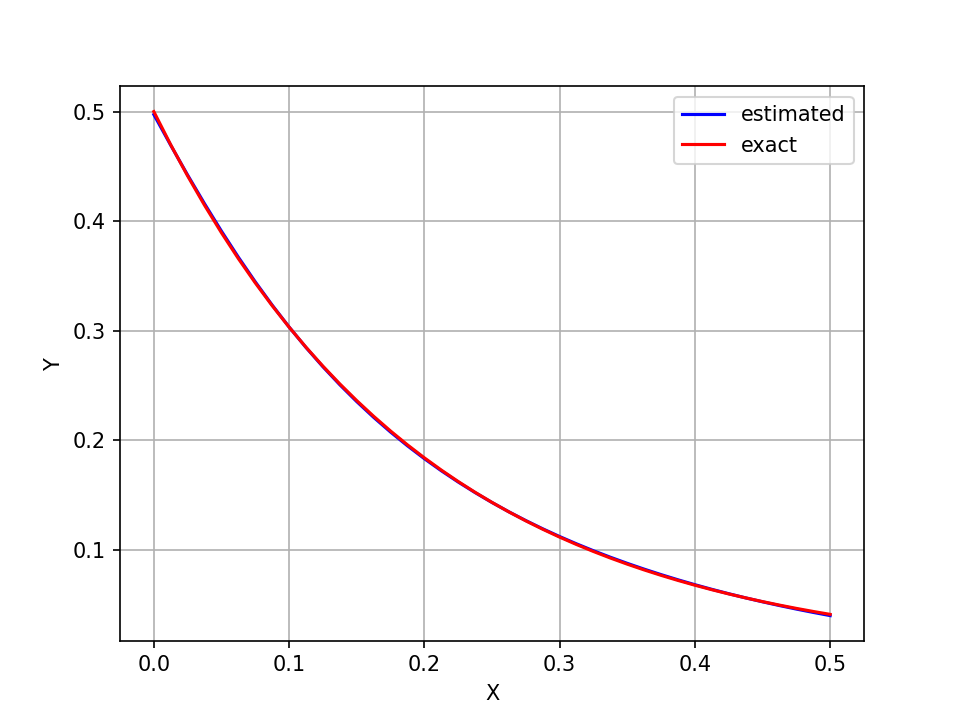
\includegraphics[scale=0.5]{supportingFiles/02_results/03_derivative_validation/estimation.png}
        \caption{Velocity profile estimated vs expected}
        \label{validation_decay_profile}
    \end{subfigure}
    \hfill
    \begin{subfigure}{0.5\linewidth}
       \center
        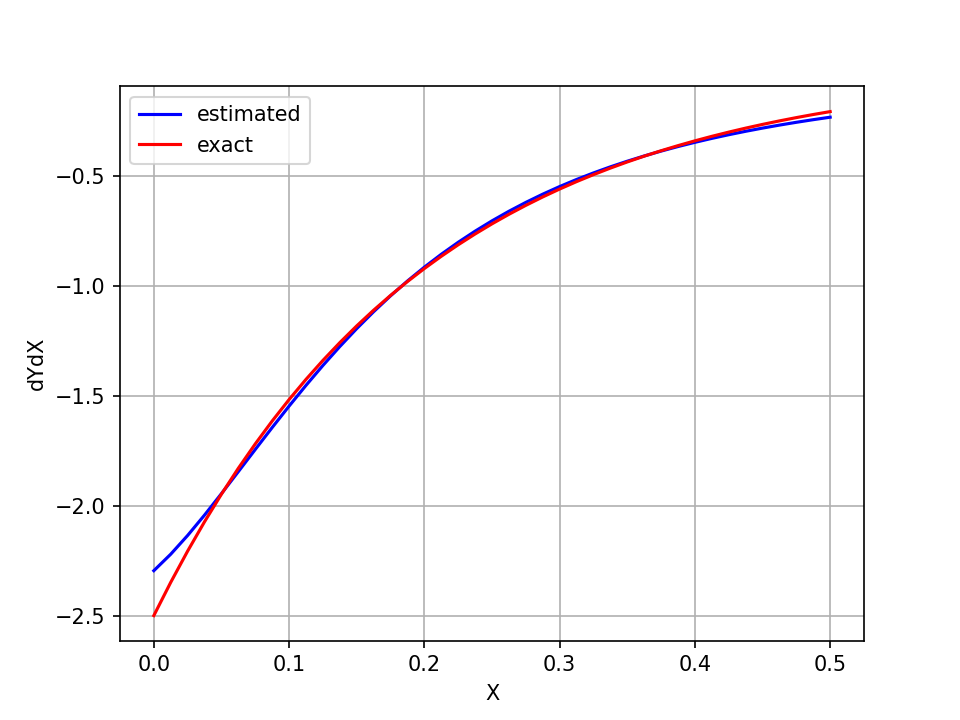
\includegraphics[scale=0.5]{supportingFiles/02_results/03_derivative_validation/derivative.png}
        \caption{\(dV/dt\) profile estimated vs expected}
        \label{validation_derivative_profile}
    \end{subfigure}
    \hfill
    \caption{Validation graphs for derivative computation}
\end{figure}

